
Welcome to Hermes2D, a high-performance $hp$-FEM PDE solver library for a wide range
of 2D problems. This manual describes how to install the library and apply it to
problems of electromagnetics, structural mechanics, fluid dynamics, and more.

The $hp$-FEM is a modern version of the Finite Element Method (FEM) which
combines elements of variable diameter $h$ and polynomial degree $p$ to obtain
extremely fast (exponential) convergence rates. Hermes2D implements quality $H^1$ and
$\Hcurl$ conforming higher-order elements and contains novel algorithms
that enable easy and modular construction of advanced, automatically-adaptive
$hp$-FEM solvers.

Hermes2D has the following features:
\begin{itemize}
  \item supports general unstructured triangular and quadrilateral meshes,
  \item handles arbitrary element refinements and irregular meshes, thus enabling
        adaptive solutions,
  \item implements curvilinear elements with edges defined by NURBS curves,
  \item allows the solution of systems of PDEs,
  \item can be used for both linear and non-linear, stationary and time dependent
        problems,
  \item enables the use of different elements ($H^1$, $\Hcurl$, $L^2$, Taylor-Hood) in
        one computation,
  \item allows each solution component to have a different mesh,
  \item implements an easy-to-use automatic $hp$-adaptivity module,
  \item contains basic postprocessing and visualization functions.
\end{itemize}

Due to the broad range of problems to which it can be applied, Hermes2D was not
designed as a~standalone program but rather as a library intended for the creation
of more specialized solvers. For example, it is almost impossible to devise
a simple yet sufficiently general input file format fully covering all problem
types mentioned above. Therefore, we expect that highly specialized front-ends to
the library will be implemented in the future; see Figure~\ref{fig:frontends}.

\begin{figure}[ht]
  \centering
  \medskip
  \includegraphics[width=0.8\textwidth]{img/frontends}
  \caption{Possible front-ends to Hermes2D.}
  \label{fig:frontends}
\end{figure}

This manual covers the steps required to develop such front-ends, which is currently
the only way to use Hermes2D. Therefore, the library may not yet be for everyone, as
its usage assumes at least a minimal knowledge of C or C++. On the other hand, the
interface to Hermes2D is quite simple and easy to learn.

As mentioned, Hermes2D is written in C++, you will therefore need a C++ compiler. The
library can be compiled with the GNU compiler ({\tt gcc}) or the Intel compiler
({\tt icc}). The default linear solver is UMFPACK. See Chapter~\ref{ch:install} for
installation instructions.

After installing, start reading Section~\ref{ch:getstart} for a quick tutorial on
using the library. Section~\ref{ch:libref} contains a detailed reference
manual and finally Section~\ref{ch:examples} provides several more advanced examples
of using Hermes2D.
